\section{La notation musicale}

\subsection{La partition}


Une partition est un document contenant toutes les informations jugées nécessaires par l'auteur pour pouvoir interpréter une musique. Elle est composée de portées qui contiennent elles-même des mesures. Une mesure dispose d'une clé, d'une armure et d'une signature si elle est la première de sa portée et une ensemble de notes, accords ou silences.

\begin{figure}[!h]
\centering

\begin{music}

\instrumentnumber{1} % nombre de voix
\generalmeter{\meterfrac{4}{4}} % mesure 4/4
%\setname 1{chant} %nom de la portée
\generalsignature{3} % armure

\startextract
\metron{\qu}{60} % tempo
\NOTes\ha g\en %une blanche
%\NOTesp\qap g\en %une blanche pointée
\NOTes\hpause \en %une demi-pause

%\bar
%\Notes \islurd0c\qu{c d e}\tslur0f\qu f \enotes %liaison

\bar
%\Notes \ibu0d0\qb0{c c c}\tbu0\qb0d \enotes %beam
\Notes\qa g\en %une croche
\notes\Dqbu fg\en %beam double
\Notes\ibbbu0h0\qb0e\tbbbu0\qb0e\tbbu0\qb0e\tbu0\qb0e\en %beam
\NOTes\zq c\zq e\zq g\qu j \en %accord
%\NOTes \zq{ceg}\qu j \en % autre manière de faire un accord

\endextract

\end{music}

\caption{Exemple d'une partition}
\end{figure}


\par
Une partition peut comporter plusieurs instruments ou voix. Une voix peut être formée de une (chant) ou deux portées (piano).

\begin{figure}[!h]
\centering

\begin{music}

\instrumentnumber{2} % 2 instruments

\setstaffs 1{2} % instrument 1 (en bas) : 2 portées

\setclef{1}{60} % clef de fa (6) en 1, clef de sol (0) en 2
\generalmeter{\meterfrac{4}{4}} % mesure 4/4
\setname 1{piano} %
\setname 2{chant} %
\parindent 10mm % pour éviter la collision de piano avec l'accolade

\startextract
% {{bleu|1re mesure}}
\Notes
\ha J | % chgt portée, même instr
\zhu{c e}\hu g & % chgt instr ; pas d'espace entre } et \hu
\ibu0d0\qb0{c c c}\tbu0\qb0d
\enotes % assure l'alignement
%
\Notes
\ha N | % chgt portée, même instr
\zhu{g i}\hu k & % chgt instr
\qa{e d}
\enotes

\bar % après toutes les notes de la mesure, pour toutes les voix
% {{bleu|2e mesure}}
\Notes
\qa J |
\zqu{c e}\qu g &
\ibu0d0\qb0{c e}
\enotes
%
\Notes
\qa N |
\zqu{g i}\qu k &
\qb0{d}\tbu0\qb0d
\enotes
%
\Notes
\ha J |
\zhu{c e}\hu g &
\ha c
\enotes
%
\endextract

\end{music}

\caption{Plusieurs portées et voix}
\end{figure}

\subsection{La durée}

La durée est le temps pendant laquelle la note est jouée. La durée n'est pas exprimée sous forme de valeur fixe mais comme une proportion relative à la mesure. En effet, la durée de la mesure dépend de sa signature et du tempo (expliqués plus tard).


\subsection{La signature}

La signature symbolise le référentiel de la durée de la mesure. Elle peut être représentée sous forme d'une fraction. Le numérateur permet de définir la durée totale de la mesure et le dénominateur la durée d'un temps dans la mesure.

\subsection{La note}

Une note est définie par sa hauteur et sa durée. La hauteur caractérise la fréquence du son d'une note. Cette fréquence est divisée en 8 intervalles appelés octave. Cette octave est divisée en 7 hauteurs : do, do\#, ré, ré\#, mi, fa, fa\#, sol, la, la\#, si et si\#. En ce qui concerne la durée de la note, elle est indiquée par la tête de la note et la présence ou non de symboles de croches. Si l'on ne prend pas en compte les croches, il existe 4 types de durées pour une note : carrée, ronde, blanche et noire. Une note carrée vaut 2 rondes, 4 blanches et 8 noires. Afin d'exprimer une durée plus courte que celle de la noire, on peut lui rajouter un ou plusieurs symboles de croches. La durée de la note s'en retrouve divisée par deux à chaque ajout.


\begin{figure}[!h]
  \centering
  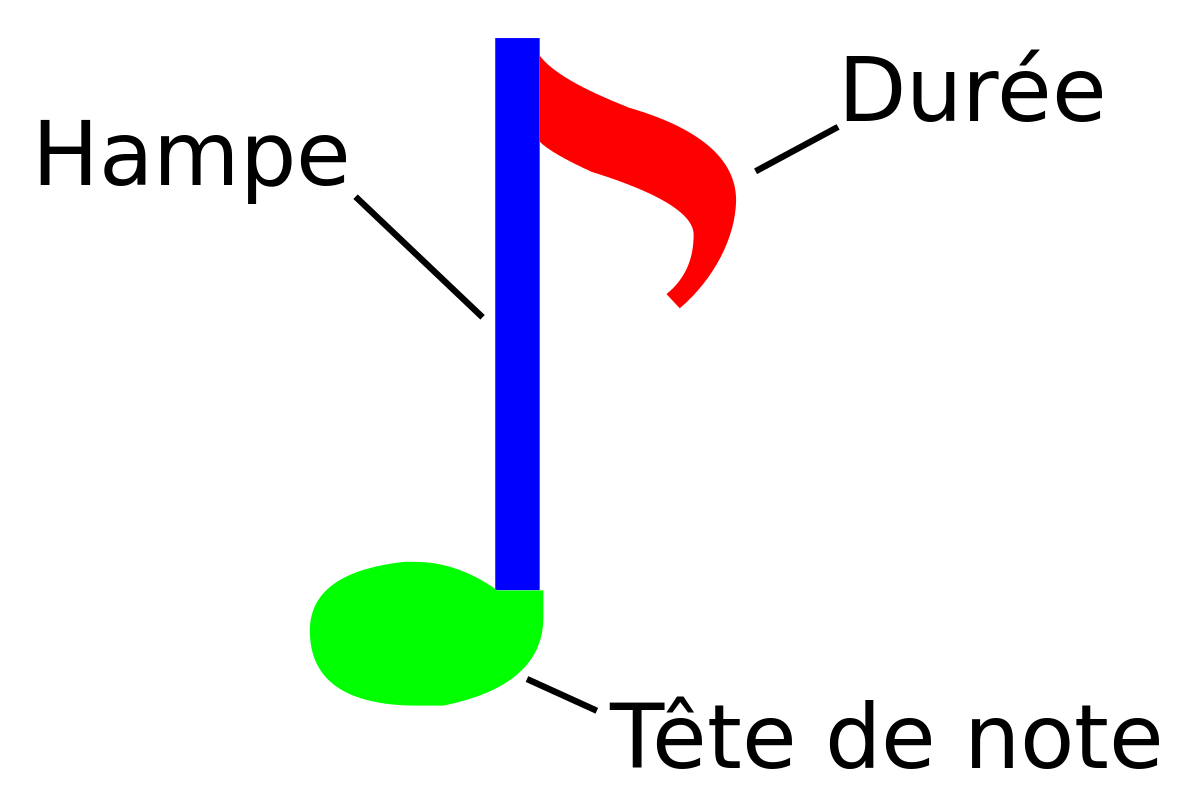
\includegraphics[width=0.3\textwidth]{note.png}\\[1cm]
  \caption{Symbole d'une note}
\end{figure}


\par
Dans notre programme, tout comme dans MusicXML, nous utilisons la notation anglo-saxonne. Elle diffère de la notation française par la façon dont est exprimée la hauteur et la durée de la note. Do, ré, mi, fa, sol, la et si sont remplacées respectivement par C, D, E, F, G, A et B. Concernant la durée, ce sont simplement des fractions. Par exemple, la blanche est un 1/2 (half) et la noire 1/4 (quarter).


\begin{figure}[!h]
\centering

\begin{music}

\instrumentnumber{1}

\startextract
\NOTes\wh g\en % rond
\NOTes\ha g\en % blanche
\NOTes\qa g\en % noire
\NOTes\ca g\en % croche
\NOTes\cca g\en % double croche
\NOTes\ccca g\en % triple croche
\NOTes\cccca g\en % quadruple croche
\endextract

\end{music}

\caption{Les différents figures de notes}
\end{figure}


\subsection{Le silence}

Un silence est un arrêt momentané dans l'exécution d'une œuvre. Tout comme les notes, il existe différentes figures de silence variant en fonction de leur durée. La pause a la même durée qu'une ronde et se situe sous la quatrième ligne de la portée. La demi-pause, d'une durée égale à la blanche, se place sur la troisième ligne. Les autres figures sont le soupir, le demi-soupir, le quart de soupir, huitième de soupir, seizième de soupir, etc. La figure suivante montre ces figures de silence.


\begin{figure}[!h]
\centering

\begin{music}

\instrumentnumber{1}

\startextract
\NOTes\pause \en % pause
\NOTes\hpause \en % demi-pause
\NOTes\soupir \en % soupir
\NOTes\ds \en % demi-soupir
\NOTes\qs \en % quart de soupir
\NOTes\hs \en % 8ème de soupir
\NOTes\qqs \en % 16ème de soupir
\endextract

\end{music}

\caption{Les différents figures de silence}
\end{figure}


\subsection{Le tempo}

Le tempo correspond à la vitesse d'exécution d'un morceau de musique. Il contient un type (une noire par exemple) et un nombre par minute. Ainsi, le tempo \emph{60 à la noire} signifie qu'il y a, dans une minute, 60 noires ou bien 30 blanches. Il se place en début de mesure mais peut parfois être absent. L'interprète peut dans ce cas jouer le morceau à la vitesse souhaité.


\subsection{Les symboles musicaux}

Nous désignons par symbole musical, chaque artefact influençant la manière de jouer une note ou un groupe de notes.

\par
Certains symboles ne s'appliquent que sur une figure de note. Ils sont dits unaires. La figure suivante montre quelques exemples de symboles unaires.

\begin{figure}[!h]
\centering

\begin{music}

\instrumentnumber{1}

\startextract
\NOTes \trrml j\ha j \en % tremolo double
\NOTes\en
\def\atnextbar{\znotes\loffset{0.7}{\centerbar{\Fermataup l\wh j}}\en}% point d'orgue

\bar
%accent
\Notes\ibu0f3\busfz0\qb0f\bupz0\qb0g\bust0\qb0h\buppz0\qb0i\busf0\qb0j\butext0\tqh0k\en
\endextract

\end{music}

\caption{Symboles unaires}
\end{figure}

\par
Les symboles influençant un groupe de notes sont appelés symboles binaires. Les 4 symboles suivant sont une liaison, un triolet, une appoggiature et un groupe de croches. Ce dernier est constitué de plusieurs croches reliées entre elles par une ou plusieurs barres selon la durée des notes. Une telle barre est appelée \emph{beam} en anglais.

\begin{figure}[!h]
\centering

\begin{music}

\instrumentnumber{1}

\startextract
\NOtes \islurd0g\qu g\tslur0g\qu g\en
\notesp \triolet n\isluru0l\Ibl0ln2\qb0{lm}\tslur0n\tqb0n\en % triolet
\notes \multnoteskip\smallvalue\smallnotesize\grcu j\en % petite note de l'appogiature
\NOTes \hu i\en
\Notes\ibbbu0h0\qb0e\tbbbu0\qb0e\tbbu0\qb0e\tbu0\qb0e\en %beam
\endextract

\end{music}

\caption{Symboles binaires}
\end{figure}


Des symboles servent à répéter les notes d'une ou de plusieurs mesures.

\begin{figure}[!h]
\centering

\begin{music}

\instrumentnumber{1}

\startextract
\NOTes\ha g\en
\leftrepeat
\NOTes\ha h\en
\leftrightrepeat
\NOTes\ha i\en
\rightrepeat
\NOTEs\wh j\en

\endextract

\end{music}

\caption{Symboles de répétitions}
\end{figure}



% \subsection{L'arbre rythmique}
%
% \par
% Dans notre application, les durées des éléments constituant les mesures sont représentées sous forme d'arbres rythmiques. Comme décrit dans l'article \cite{agon}, \enquote{un arbre rythmique est défini comme un couple (D S) où D est une fraction (< 0) et S est une liste de n-éléments définissant n-proportions de D. Chaque élément de S peut-être soit un entier, soit un arbre rythmique.}
%
% \par
% Si S est une note, l'entier aura une valeur positive, si c'est un silence, il sera négatif. Si il y a une liaison, la note qui la termine a une valeur flottante (e.g. 1.0). Dans le couple, la valeur de la note de plus courte durée sera de 1, les valeurs des notes ayant une plus longue durée seront proportionnelles à celle-ci.
%
% \par
% Le couple (D S) peut être représenté sous forme arborescente. La fraction D est située à la racine. Les éléments de S sont donc les nœuds ou les feuilles.
%
% \par
% Soit la partition suivante, constituée d'une blanche, de deux noires reliées par une liaison et d'un soupir :
%
% \begin{music}
%
% \instrumentnumber{1}
% \generalmeter{\meterfrac{5}{4}}
%
% \startextract
% \NOTes\ha g\en
% \NOtes \islurd0g\qu g\tslur0g\qu g\en
% \NOTes\soupir \en
% \endextract
%
% \end{music}
%
% Le couple (D S) peut donc être représenté des manières suivantes :
%
% \begin{center}
% (5/4 (2 1 1.0 -1) )
% \end{center}
%
% \begin{figure}[!h]
% \Tree[.5/4 [.2 ]
%            [.1 ]
%            [.1.0 ]
%            [.-1 ]
%      ]
%
% \caption{Arbre rythmique 1}
% \end{figure}
%
%
%
% \par
% Prenons une autre partition contenant un triolet. Un triolet est composé de 3 figures égales, mais dont la durée en vaut deux.
%
% \begin{music}
%
% \input musixps
% \instrumentnumber{1}
% \generalmeter{\meterfrac{4}{4}}
%
% \startextract
% \NOTes\qa g\en
% \notesp\triolet n\Ibl0ln2\qb0{ll}\tqb0n \en % triolet
% \NOTes\ha g\en
% \endextract
%
% \end{music}
%
% Le couple (D S) et l'arbre rythmique correspondant sont :
%
% \begin{center}
% (4/4 (1 (1 (1 1 1) ) 2) )
% \end{center}
%
% \begin{figure}[!h]
% \Tree[.4/4 [.1 ]
%            [.1
%                [.1 ]
%                [.1 ]
%                [.1 ]
%            ]
%            [.2 ]
%      ]
%
% \caption{Arbre rythmique 2}
% \end{figure}
%
%

%rt de silence et liaison
